%!TEX root = ../template.tex
%%%%%%%%%%%%%%%%%%%%%%%%%%%%%%%%%%%%%%%%%%%%%%%%%%%%%%%%%%%%%%%%%%%
%% chapter1.tex
%% NOVA thesis document file
%%
%% Chapter with introduciton
%%%%%%%%%%%%%%%%%%%%%%%%%%%%%%%%%%%%%%%%%%%%%%%%%%%%%%%%%%%%%%%%%%%
\newcommand{\novathesis}{\emph{novathesis}}
\newcommand{\novathesisclass}{\texttt{novathesis.cls}}

%In general, molecular docking involves two steps: global (local) search and scoring.
%In the first stage, the proteins are usually treated as rigid bodies, and one of them is kept fixed
%while the other is free to rotate and translate, searching the six-dimensional space for the candidate
%complexes. These structures are evaluated by a simple scoring function, based mainly on shape
%complementarity, in order to reduce the number of models to analyze. The second stage scores the
%candidate models using several parameters, including statistics of residue-residue contacts across
%interfaces of complexes [20,21], electrostatics, hydrogen bonding, change in accessible solvent area,
%and lack of buried charges [13]. This scoring function is meant to indicate how well the candidate
%model corresponds to the real complex. \cite{}
\chapter{Introdução}
\label{cap1}
\section{Enquadramento e motivação}
%While the structures of many protein-protein complexes have been characterized experimentally via x-ray crystallography and deposited in the Protein Data Bank (PDB; [1]), the majority of known complexes have not, providing an opportunity for predictive computational techniques to help elucidate these structures. \cite{ZDOCKaccelerating}
%O que os investigadores verificaram foi que, quando a proteína S100B interage com a proteína beta-amilóide, há um atraso na formação dos agregados de beta-amilóide, que levam posteriormente à formação das placas senis. “Estudos em culturas de células revelam que a proteína S100B reverte a toxicidade causada pelos agregados da proteína beta-amilóide”, acrescenta Cláudio Gomes. Para o investigador, isto pode significar que a proteína S1000B atua contra a formação dos agregados.

Estudar as interações entre as proteinas tem garantido avanços na descoberta de formas de proteger o Homem de doenças consideradas incuráveis. Um exemplo a considerar foi em 2018 um investigador português ter descoberto que a interação entre as proteinas S100B e beta-amiloide provocam um atraso na formação dos agregados do beta-amiloide, trazendo como beneficio a proteção contra a doença de Alzheimer\cite{noticia}. Estudar estas interações trouxe igualmente avanços consideráveis no desenho de drogas assistido por computador. Neste caso as interações a considerar são entre uma proteina e outra de dimensões menores.\par
Segundo \cite{ZDOCKaccelerating} a maioria dos complexos de proteinas ainda não foram adicionados à base de dados sobre as proteinas (PDB), que contem apenas os complexos descobertos através cristalografia por raio x. Pelo que existe a possibilidade de usar técnicas de computação para docking na elucidação de estruturas que não constem na PDB, adicionando-as a esta.
\par
O tema desta preparação está enquadrado nas áreas de bio-informática e de informática. Bio-informática no sentido de envolver conceitos relacionados com o estudo das interações entre proteinas e informática devido à parte do uso do GPU para melhorar a performance do BiGGER.
%As interações entre proteinas 
%Introduzir a noticia 
\section{Formulação do problema}
%The molecular structure of a protein-protein complex can be difficult to determine by either
%X-ray crystallography or NMR spectroscopy, especially those with a transient nature. However,
%molecular docking procedures can be used to obtain a model structure of the complex when the atomic
%coordinates of the individual proteins are known.  

\subsection{Conceito de docking}
De acordo com \cite{halperin}, docking pode ser visto como um conjunto de passos computacionais a desenvolver para determinar o melhor encaixe entre duas moléculas, sendo elas o receptor e o ligando como está ilustrado gráficamente na figura \ref{dockGraf}. Existem duas vertentes de docking, o docking vinculado (\textit{bounded docking}) aplica os passos computacionais referidos anteriormente na determinação do melhor encaixe através das estruturas vinculadas do par. Esta vertente de docking é computacionalmente mais simples do que o docking não-vinculado (\textit{unbounded docking}), onde a computação é semelhante à do docking vinculado mas a determinação do melhor encaixe é obtida através das estruturas não-vinculadas. O docking não-vinculado é também conhecido como docking predictivo, sendo a abordagem mais pretendida porém computacionalmente mais complicada. \par
O problema associado ao docking consiste em duas partes: desenvolver uma função de score que consegue discriminar com a maior precisão as orientações do ligando optimais das que não optimais.  A segunda é determinar um método de pesquisa global que consiga determinar qual das orientações corretas a melhor \cite{prediction}. \par
 Docking de proteinas consiste em prever a estrutura tri-dimensional do complexo de proteinas através das coordenadas atómicas do ligando e do receptor, consistindo em duas fases. Na fase de pesquisa global, as proteinas são consideradas como sendo corpos rigidos, o receptor fica estático e ao ligando são aplicadas rotações e translações, sendo determinados os complexos candidatos. O passo final desta fase é avaliar os candidatos encontrados através da função de score baseada na complementaridade de superficie. A avaliação é feita por uma abstração da molécula numa grelha tri-dimensional, e determinando para cada célula da grelha, se existe correspondência com uma coordenada atómica da molécula. A segunda fase consiste na atribuição de pontuação aos candidatos resultantes da fase anterior, através de uma função de score com parametros como contactos residuais, eletroestática até dissolvação. A gama de parametros tem a ver com as caracteristicas biológicas do par candidato. Esta fase permite averiguar de que forma o par candidato é correspondido com o par real\cite{bigger2016}.
\subsection{Tipos de Interações}
Existem dois tipos de interações a considerar: interações entre dois pares de proteinas (PPI) e interações entre uma proteina e uma molécula de dimensões pequenas (PDI).
\begin{figure}[ht]
  \centering
    {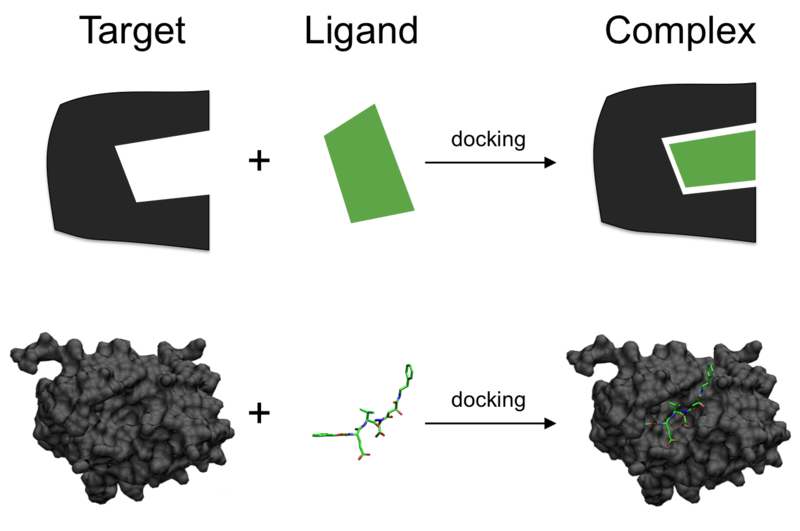
\includegraphics[width=0.5\linewidth]{Docking_representation_2}}
  \caption{Representação gráfica do docking\cite{dockingWiki}.}
  \label{dockGraf}
\end{figure}
\section{Objectivos a alcançar na elaboração da dissertação}
Assumindo que a preparação tem condições para avançar para a fase de elaboração, o objetivo desta dissertação é implementar a aceleração do algoritmo BiGGER. Esta aceleração terá de trazer à versão futura do BiGGER ganhos de speedup consideráveis em relação à versão actual que apenas usa um \textit{core} do CPU. O resultado final terá será uma versão do BiGGER que garanta uma alternativa mais eficiente em termos de computação e tempo de execução face aos restantes algoritmos de docking de proteinas.
\section{Estrutura deste documento}
O presente documento de preparação assume três capítulos:
\begin{enumerate}
\item{Introdução}
\item{Estado da arte}
\item{Plano de trabalho}
\end{enumerate}
%Os seguintes pontos abordam ferramentas para docking que surgiram antes do aparecimento do conceito introduzido em \ref{gpus}, sendo as respetivas formas de docking relacionadas com a do BiGGER. A diferença entre as ferramentas indicadas nesta secção e as presentes na secção \ref{}

O capítulo \ref{cap1} é feita a uma introdução sobre os conceitos de docking a ter em conta assim como uma formulação do problema computacional associado ao mesmo. No capítulo \ref{cap2} é feita uma visão geral em relação aos diversos métodos e ferramentas de docking, inclusive o BiGGER, indicando as diferenças em relação a este último. Estas ferramentas surgiram antes de ser considerado o GPU para acelerar o docking. Neste capítulo também está incluido uma secção em que é abordado os conceitos associados ao GPU e respetiva programação, assim como o que é que existe em termos de software especifico para docking com acelerações em GPU relacionado com o BiGGER. Como foi implementada essa aceleração e de que forma é que é util para a aceleração do BiGGER. Também são abordados duas APIs para programação em GPU: CUDA e OpenCL.
Por fim no capítulo \ref{cha3}, é descrito o estado de performance da versão actual do BiGGER, através dos resultados do profiling feito a este. Estes resultados permitem definir as zonas de código do programa que precisam de ser acelerados por GPU e por consequência o plano de trabalho para os acelerar. Aborda-se ainda duas possiveis ramificações sobre como implementar os mecanismos de aceleração ao BiGGER assim como os aspetos positivos e os negativos de ambas. 


%\begin{quotation}
%  \itshape
%  This work is licensed under the Creative Commons Attribution-NonCommercial~4.0 International License.
%  To view a copy of this license, visit \url{http://creativecommons.org/licenses/by-nc/4.0/}.
%\end{quotation}


%\section{A Bit of History} % (fold)
%\label{sec:a_bit_of_history}
%
%The \novathesis\ was originally developed to help MSc and PhD students of the Computer Science and Engineering Department of the Faculty of Sciences and Technology of NOVA University of Lisbon (DI-FCT-NOVA) to write their thesis and dissertations Using \LaTeX.
%%
%These student can easily cope with \LaTeX\ by themselves, and the only need some help in the bootstrap process to make their life easier.
%
%However, as the template spread out among the students from other degrees at FCT-NOVA, the demand for am easier-to-use template as grown.
%%
%And the template in its current shape aims at answering the expectations of those that, although they are not familiar with programming nor with markup languages, so still feel brave enough to give \LaTeX\ a try and rejoice with the beauty of the texts typeset by this system.
% 
%% section a_bit_of_history (end)
%
%
%\section{Disclaimer} % (fold)
%\label{sec:disclaimer}
%
%It is up to you, the student, to read the FCT and/or NOVA regulations on how to format and submit your MSc or PhD dissertation.  
%
%This template is endorsed by the FCT-NOVA and even linked from its web pages, but it is not an official template.
%%
%This template exists to make your life easier, but in the end of the line you are accountable for both the looks and the contents of the document you submit as your dissertation.

